\documentclass[12pt,xcolor=table]{beamer}
% Russian
\usepackage[english]{babel}
\usepackage{fontspec}

% Use font with cyrillic characters
\setmainfont{Open Sans}
\setsansfont{Open Sans}
\setmonofont{Inconsolata}

% Various packages
\usepackage{graphicx}
\usepackage{xcolor}
\usepackage{svg}
\usepackage{multirow}
\usepackage{xparse}
\usepackage{listings}

% Include TOC before each frame
\AtBeginSection[]{\begin{frame}<beamer>\frametitle{}\tableofcontents[currentsection,hideothersubsections]\end{frame}}

% Minted package for code listings
\usepackage{minted}
\setminted[bash]{
    frame=lines,
    framesep=2mm,
    baselinestretch=1.2,
    fontsize=\footnotesize,
    linenos
}
\graphicspath{ {./images/} }
\usepackage{hyperref}

\title{Introduction to GraphQL}
\subtitle{\url{https://github.com/anak10thn}}
\date{8 April 2023}

\usecolortheme[named=teal]{structure}

\begin{document}

\maketitle

\begin{frame}
\frametitle{Overview}
\tableofcontents
\end{frame}

\section{Apa itu GraphQL}

\begin{frame}
\begin{itemize}
    \item Dibuat oleh facebook pada 2012 dan diopen sourcekan pada 2015.
    \item Declarative Query language yang memungkinan client melakukan request data yang diinginkan dari server.
    \item Backend for Frontend (BFF) pattern.
    \item Struktur data non-linier yang memiliki nodes \& edges.
\end{itemize}
\end{frame}

\section{Persepsi keliru tentang GraphQL}

\begin{frame}
\begin{itemize}
    \item \textbf{GraphQL sebagai pengganti RestAPI.} \textit{Kenyataannya GraphQL menggunakan RestAPI untuk mengirim Query request keserver.}
    \item \textbf{GraphQL adalah bahasa untuk query database.} \textit{Kenyataannya GraphQL tidak bisa melakukan query ke database.}
    \item \textbf{GraphQL adalah sebuah teknologi.} \textit{GraphQL bukan sebuah teknologi melainkan sebuah pattern.}
\end{itemize}
\end{frame}

\section{Siapa yang menggunakan?}
\begin{frame}

\includegraphics[scale=0.3]{images/who-use-it.png}
\url{https://graphql.org/users}
\end{frame}

\section{Kenapa GraphQL?}

\begin{frame}
\frametitle{Rest API}
\begin{columns}
\begin{column}{0.6\textwidth}
    \begin{itemize}
        \item Satu API call untuk menampilkan list item.
        \item Beberapa API call untuk menampilkan detail masing-masing item.
        \item Under-fetching dan Over-fetching
    \end{itemize}
\end{column}
\begin{column}{0.4\textwidth}  %%<--- here
    \inputminted{bash}{code/rest.text}
    \textit{O(n+1)}
\end{column}
\end{columns}
\end{frame}

\begin{frame}
\frametitle{GraphQL}
\begin{columns}
\begin{column}{0.6\textwidth}
    \begin{itemize}
        \item \textbf{Meminimalisir Under-fetching dan Over-fetching.}
        \item \textbf{Strongly type schema}
            \begin{itemize}
                \item Schema dapat digunakan di client dan server.
                \item Request dapat dengan mudah divalidasi.
                \item Auto complete query dan mutation.
                \item Sangat mudah di mocked.
            \end{itemize}
    \end{itemize}
\end{column}
\begin{column}{0.4\textwidth}  %%<--- here
    \inputminted{bash}{code/graphql.text}
    \textit{O(1)}
\end{column}
\end{columns}
\end{frame}


\section{GraphQL Operation}

\begin{frame}
\underline{Queries}

\scriptsize\textit{Read data}
\inputminted{bash}{code/query.text}
\end{frame}

\begin{frame}

\underline{Mutations}

\scriptsize\textit{Write data}
\inputminted{bash}{code/mutation.text}

\end{frame}

\begin{frame}
\underline{Subscriptions}

\scriptsize\textit{Listen for data}
\inputminted{bash}{code/subscribe.text}
\end{frame}

\section{Schema Definition Language (SDL) Type}

\begin{frame}
\frametitle{Object Types}
\inputminted{bash}{code/object.text}
\end{frame}

\begin{frame}
\frametitle{Scalars}
\begin{itemize}
    \item String
    \item Float
    \item Int
    \item Boolean
    \item ID
    \item Custome scalars e.g. Date, Email
\end{itemize}
\end{frame}

\begin{frame}
\frametitle{Enum}
\inputminted{bash}{code/enum.text}
\end{frame}

\begin{frame}
\frametitle{Enum}
\inputminted{bash}{code/objectenum.text}
\end{frame}

\begin{frame}
\frametitle{Type Modifier}
\begin{itemize}\small
    \item \text{String: nullable string.}
    \item \text{String!: Non-nullable string.}
    \item \text{[String]: Nullable list of nullable string values.}
    \item \text{[String!]: Nullable list of non-nullable string values.}
    \item \text{[String!]!: Non-nullable list of non-nullable string values.}
\end{itemize}
\end{frame}

\section{Tools & Library}

\begin{frame}
\frametitle{Library}
\begin{itemize}\small
    \item \href{https://github.com/async-graphql/async-graphql}{Async GraphQL} (Rust)
    \item \href{http://graphene-python.org/}{Graphene} (Python)
    \item \href{https://github.com/graphql-java/graphql-java}{GraphQL Java} (Java/Kotlin)
    \item \href{https://github.com/graphql-go/graphql}{GraphQL Go} (Go)
    \item \href{https://graphql.org/graphql-js/}{GraphQL.js} (javascript)
\end{itemize}
\end{frame}

\begin{frame}
\frametitle{Playground}
\begin{itemize}\small
    \item \href{https://altairgraphql.dev/}{Altair GraphQL}
    \item \href{https://www.graphqlbin.com/v2/new}{GraphQL Bin}
    \item \href{https://github.com/graphql/graphql-playground}{GraphQL IDE}
\end{itemize}
\end{frame}

\begin{frame}
\frametitle{Framework \& Gateway}
\begin{itemize}\small
    \item \href{https://typegraphql.com/}{Type GraphQL}
    \item \href{https://github.com/graphteon/remora}{Remora}
    \item \href{https://github.com/graphteon/shark}{Shark}
\end{itemize}
\end{frame}

\begin{frame}
\frametitle{Remora}
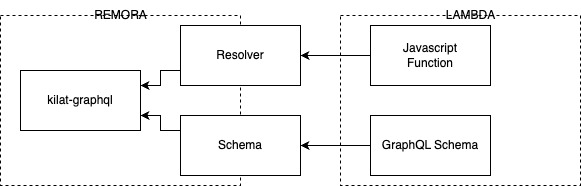
\includegraphics[scale=0.5]{images/remora.jpeg}
\url{https://github.com/graphteon/remora}
\end{frame}

\begin{frame}
\frametitle{Shark}
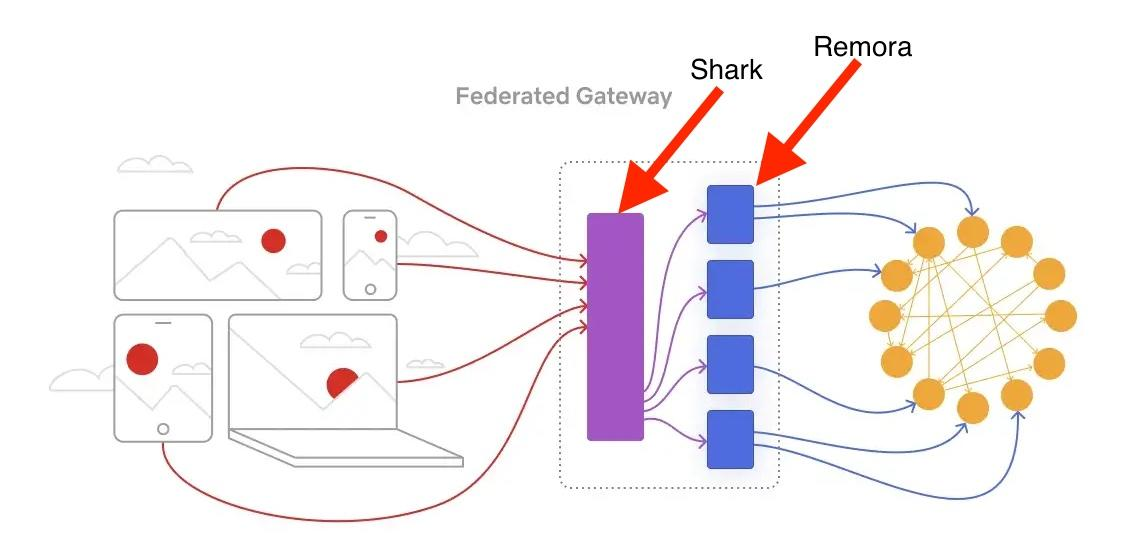
\includegraphics[scale=0.3]{images/shark.jpeg}
\url{https://github.com/graphteon/shark}
\end{frame}

\section{Demo}

\end{document}